\documentclass[tikz, margin=3mm]{standalone}
\usepackage[utf8]{inputenc}
\usepackage{tikz}
\usetikzlibrary{shapes.geometric, arrows, calc}

\makeatletter
\newcommand{\gettikzxy}[3]{%
  \tikz@scan@one@point\pgfutil@firstofone#1\relax
  \edef#2{\the\pgf@x}%
  \edef#3{\the\pgf@y}%
}
\makeatother



\tikzstyle{startstop} = [rectangle, rounded corners, minimum width=3cm, minimum height=1cm,text centered, draw=black, fill=red!30]
\tikzstyle{io} = [trapezium, trapezium left angle=70, trapezium right angle=110, minimum width=3cm, minimum height=1cm, text centered, draw=black, fill=blue!30]
\tikzstyle{process} = [rectangle, minimum width=3cm, minimum height=1cm, text centered, draw=black, fill=orange!30]
\tikzstyle{decision} = [diamond, minimum width=3cm, minimum height=1cm, text centered, draw=black, fill=green!30]

\tikzstyle{arrow} = [thick,->,>=stealth]


\begin{document}


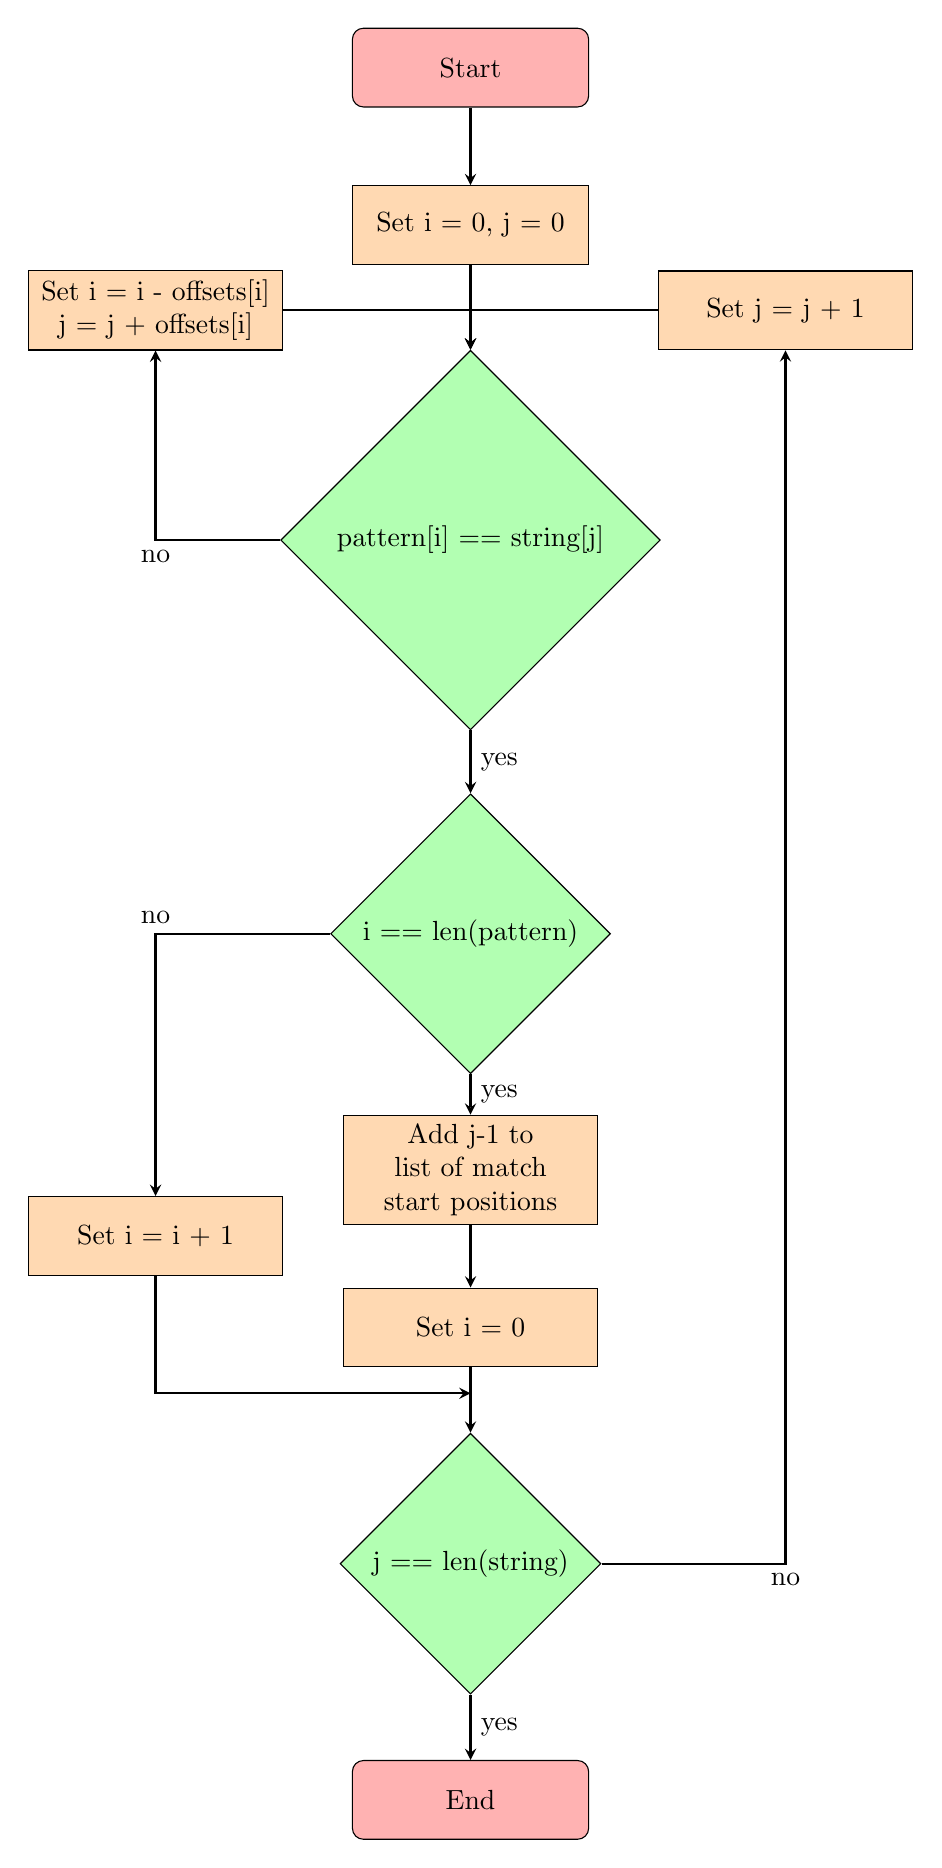
\begin{tikzpicture}[node distance=2cm]
    \node (start) [startstop] {Start};
    \node (set_i_j) [process, below of=start] {Set i = 0, j = 0};
    \node (pattern_string) [decision, below of=set_i_j, text width=4cm, yshift=-2cm] {pattern[i] == string[j]};

    \coordinate (coord0) at ($(pattern_string.north)+(0,0.5cm)$);
    \node (set_i_j2) [process, left of=coord0, text width=3cm, xshift=-2cm] {Set i = i - offsets[i] j = j + offsets[i]};
    \node (set_j) [process, right of=coord0, text width=3cm, xshift=2cm] {Set j = j + 1};


    \node (i_len) [decision, below of=pattern_string, yshift=-3cm] {i == len(pattern)};
    \node (add) [process, below of=i_len, yshift=-1cm, text width=3cm] {Add j-1 to list of match start positions};
    \node (set_i) [process, below of=add, text width=3cm] {Set i = 0};
    \node (j_len) [decision, below of=set_i, yshift=-1cm] {j == len(string)};

    \coordinate (coord1) at ($(j_len.north)+(0,0.5cm)$);
    \node (set_i_2) [process, left of=coord1, text width=3cm, xshift=-2cm, yshift=2cm] {Set i = i + 1};

    \node (end) [startstop, below of=j_len, yshift=-1cm] {End};

    \draw [arrow] (start) -- (set_i_j);
    \draw [arrow] (set_i_j) -- (pattern_string);
    \draw [arrow] (pattern_string) -- node[anchor=west] {yes} (i_len);
    \draw [arrow] (i_len) -- node[anchor=west] {yes} (add);
    \draw [arrow] (add) -- (set_i);
    \draw [arrow] (set_i) -- (j_len);
    \draw [arrow] (j_len) -- node[anchor=west] {yes} (end);

    \draw [arrow] (set_i_j2) -- (coord0) -- (pattern_string);
    \draw [arrow] (set_j) -- (coord0) -- (pattern_string);

    \draw [arrow] (j_len) -| node[anchor=north] {no} (set_j);
    \draw [arrow] (i_len) -| node[anchor=south] {no} (set_i_2);
    \draw [arrow] (pattern_string) -| node[anchor=north] {no} (set_i_j2);
    \draw [arrow] (set_i_2) |- (coord1);

\end{tikzpicture}


\end{document}

